\documentclass{beamer}

\usetheme{Warsaw}

\title{Level 4 Project Presentation \\ A lightweight protocol for constrained devices for use in the Internet of
Things paradigm}
\author{Fergus Leahy}


\begin{document}
\maketitle


\begin{frame}
  \frametitle{Overview}
  \tableofcontents{}
\end{frame}


\section{What is the Internet of Things?} % (fold)
  \label{sec:introduction}
  \begin{frame}[t]\frametitle{What is the Internet of Things?}
    \begin{itemize}
      \item [--] \textbf{1999: RFID}
      \begin{itemize}
        \item Originally coined by Kevin Ashton, when managing company supply chain using RFID in 1999.
        \item Never really took off.
      \end{itemize}
    \end{itemize}
  	\begin{itemize}
      \item[--] \textbf{2013: Year of Internet of Things}
      \begin{itemize}
        \item Advent of cheap, low-power and small constrained devices.
        \item Consumer Electronics Show 2013
        \item Hobbyists + micro-controllers
        \item Smart fridges, Smart watches, Smart washing machines, Smart scales, Smart cars, Smart Things and Smart ... plants?
        \item Plug something into the Internet, it's now smart.
        \item Creates an Internet of Things which can notify you when your wash cycle has complete, your milk has gone off and your plants about to bite the dust.
      \end{itemize}
    \end{itemize}

    \begin{figure}[htb]
    \begin{minipage}{0.3\textwidth}
      \centering
        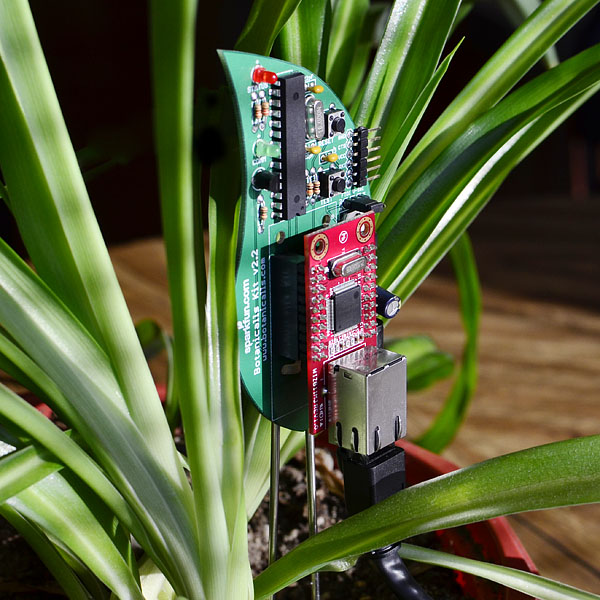
\includegraphics[scale=0.45]{presentation/img/smart-plant.jpg}
      \end{minipage}%
      \begin{minipage}{0.3\textwidth}
        \centering
          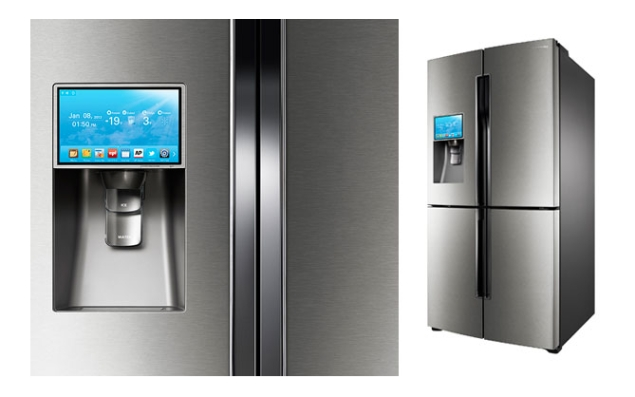
\includegraphics[scale=0.2]{presentation/img/smart-fridge.jpg}
      \end{minipage}%
      \begin{minipage}{0.3\textwidth}
        \centering
          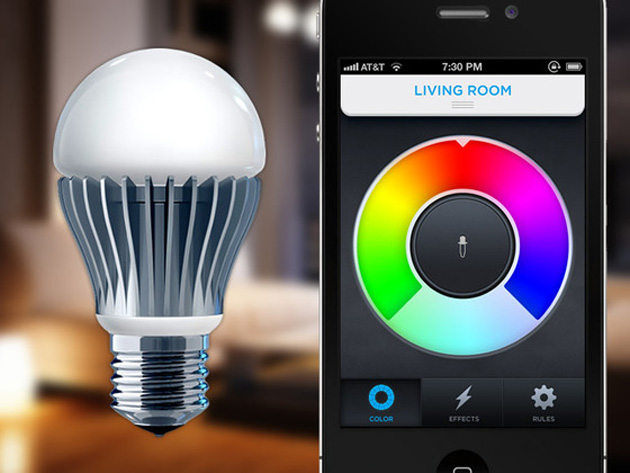
\includegraphics[scale=0.1]{presentation/img/smart-light.jpg}
      \end{minipage}
    \end{figure}
  \end{frame}

  \begin{frame}[t]\frametitle{The bigger picture}
  \begin{itemize}
    \item Combine these cheap, small individual Things to create an autonomous network of devices.
    \item A network of devices which can sense, think and react to the environment.
    \item Relates to Wireless Sensor networks.
    \item More than just singular, simple actions, e.g.,
    \begin{itemize}
      \item Alarm set for 7.30AM, coffee machines turns on, blinds slowly open.
      \item House sensing user location, adjusting lighting and heating.
      \item Plants automatically watered based on soil moisture, weather patterns. 
    \end{itemize}
  \end{itemize}
  \end{frame}

\begin{frame}[t]\frametitle{Why?}
\begin{itemize}
  \item [--] \textbf{Not just a case of being lazy...}
  \item [--] \textbf{The Internet of People}
\begin{itemize}
  \item Internet in 2009 was 500 exabytes (that's 500 BILLION gigabytes), of which 70\% was contributed to by users
  \item Users are bad at data entry.
  \item Devices are reliable and accurate.
\end{itemize}
\item [--] \textbf{Smarter decisions = Savings}
  \begin{itemize}
    \item Complex decisions based on lots of data.
    \item Efficient use of resources.
    \item Saving the user money, and the world.
  \end{itemize}
\end{itemize}
\end{frame}


\section{What's wrong?} % (fold)
\begin{frame}[t]\frametitle{What's wrong, hasn't this been solved already?}
\label{sec:what_s_wrong_}
\begin{itemize}
  \item [--] \textbf{Eco-system is full of individual Things}
  \begin{itemize}
    \item Manufacturers' own standards, non-compliant
    \item Heterogeneous devices, no easy way of connecting all devices efficiently
    \item Simple devices, limited connectivity
  \end{itemize}
\item [--] \textbf{Not really...not yet}
  \begin{itemize}
    \item Manufacturers only creating proprietary tech.
    \item Crowd-funding platform Kickstarter is full of ``Things''
    \item Some open source efforts are trying...xAP, SmartThings
    \item Existing protocols are too heavyweight/un-suited to constrained devices: JMS, TCP, HTTP,etc
    \item IETF are pushing through new standards, CoRE \& CoAP, early days
  \end{itemize}
  \item [--] \textbf{No simple, scalable solution for connecting these cheap devices together}
\end{itemize}
\end{frame}

\begin{frame}[t]\frametitle{Example attempts}

\begin{itemize}
    \item [--] \textbf{xAP: eXtensible Application Protocol}
  \begin{itemize}
    \item Heterogeneous network of devices can easily join, listen in and respond to what they're interested in.
    \item Distributed architecture, no central point of failure.
    \item Devices can easily join a network.
    \item Built on top of a multicast unreliable network.
    \item Devices broadcast ALL data, limited scalability.
  \end{itemize}
  \item [--] \textbf{SmartThings}
  \begin{itemize}
    \item Making existing objects smart by connecting them to a hub wirelessly (Zigbee)
    \item Creating apps for your everyday things, user intervention.
    \item Cloud first, devices ``wired'' together in the cloud, hub just a gateway.
    \item Reliability \& Security...
    \item Yet to really open source the project
  \end{itemize}
\end{itemize}
\end{frame}
% section what_s_wrong_ (end)

\section{How can it be solved?} % (fold)
\label{sec:how_to_solve_it}
\begin{frame}[t]\frametitle{A new protocol}
\begin{itemize}
  \item [--] \textbf{Create a lightweight protocol}
  \item [--] \textbf{Break the Internet of Things down to three basic roles}
  \begin{itemize}
    \item Sensor, the see-er
    \item Actuator, the do-er
    \item Controller, the brains
  \end{itemize}
  \item [--] \textbf{Distributed architecture with selective broadcasting. Why?}
  \begin{itemize}
    \item IoT is distributed, difficult to centralise.
    \item No central point of failure.
    \item Broadcast needed for discovering devices.
  \end{itemize}
  \item [--] \textbf{Use an un-reliable connection and build reliability selectively on top. Why?}
  \begin{itemize}
    \item Full reliability e.g., TCP, is heavyweight
    \item Ephemeral data
  \end{itemize}
\end{itemize}
\end{frame}
% section how_to_solve_it (end)

\section{Comparison} % (fold)
\label{sec:comparison}

% section comparison (end)

\section{Is this it?} % (fold)
\label{sec:is_this_it_}

% section is_this_it_ (end)
\end{document}